\section{Experiments} \label{sec:experiments}

In this section, we empirically evaluate the proposed methods on image classification tasks, both separately and in combination. We first describe the experimental setup, including the data augmentation, input encoding and output decoding schemes. The metrics and baselines are
 then detailed. 
 We  present results on learned connections (\cref{sec:exp_connection}), the convolutional architecture (\cref{sec:exp_convolution}), and the adaptive discretization strategy (\cref{sec:exp_discretization}), building up to the final combined results (\cref{sec:exp_main}).

\paragraph{Setup} We evaluate our method on \mnist \citep{lecun1998gradient} and \cifar \citep{krizhevsky2009learning}. For \mnist, we round the floating-point pixels to the 
closest Boolean values,
and apply random rotations (up to $15^\circ$) and random affine transformations
 (with translations up to $10\%$ of the image size in both spatial directions) as 
 data augmentation during training. On \cifar, we use thermometer encoding with equal thresholds (c.f. \cref{sec:background})
 to convert floating-point pixels to Boolean strings
 with various lengths, following  \citet{petersen2022deep,petersen2024convolutional}; for convolutional networks, we concatenate these
Boolean strings
 along the channel dimension. Random horizontal flips and random crops of size $32 \times 32$ with a padding of 2 pixels are applied during training. No data augmentation is applied at inference on both datasets. The population count decoder as described in \cref{sec:background} is applied on both datasets. Further experimental details are included in \cref{app:exp_details}.

\paragraph{Metrics} We use test accuracy as the performance metric. To measure the Boolean circuit size, we use two metrics: the number of neurons in the Boolean network (\emph{\#neurons}), and the number of Boolean operations in the pruned Boolean circuit (\emph{\#BOPs}). 
The pruning simply removes all redundant neurons that
have no contribution to the final output,
 and removes Identity and NOT neurons by rewiring their input connections to their output connections (see \cref{app:pruning_algorithm} for details). 
We note that more advanced logic synthesis methods \citep{Mishchenko2006_DAGAwareRewriting, Brayton2010_ABC, Riener2019_OnTheFlyDAGAware, Li2024_DAGAwareSynthesisOrchestration} 
can be applied to 
further reduce the circuit size after pruning; we apply the simplest pruning to avoid bias towards any specific circuit optimization method. 
We remark that since all baselines and our method are not trained with circuit optimization in the loop, the relative comparisons before and after pruning (\ie \#neurons and \#BOPs) are similar for our empirical studies. 
Therefore, we expect the relative performance gain of our method over baselines to hold as well after applying more advanced logic synthesis techniques.

\paragraph{Baselines} For the connection learning and convolution design, we compare against DiffLogicNet \citep{petersen2022deep} and TreeLogicNet \citep{petersen2024convolutional}, respectively. 
We take the official implementation for DiffLogicNet, and the community implementation that 
matches the results reported in \citet{petersen2024convolutional} for TreeLogicNet (see \cref{app:convlogic} for details) since the official implementation is not publicly available. 
For the adaptive discretization, we compare against Gumbel noise injection \citep{yousefi2025mind} with the official implementation. 
We apply the same input encoding, output decoding, data augmentation, and model optimizer across all methods for fair comparison.

\subsection{Connection Learning} \label{sec:exp_connection}

We focus on evaluating the effectiveness of the proposed connection learning method in \cref{sec:learning_connectivity}. 
Specifically, we compare our models against DiffLogicNet, under strictly identical conditions, including network architecture (except the parameterization) and data processing.

\paragraph{Main Results} The results on \mnist and \cifar are summarized in \cref{tb:DLGN_MNIST} and \cref{tb:DLGN_CIFAR}, respectively. Across all datasets and model sizes, learned connections consistently outperform DiffLogicNet which uses fixed connections. 
Notably, on \cifar, our method uses only 512K neurons to achieve better accuracy than DiffLogicNet with twice the number of neurons (1.28M). 
On average, models with our connection learning
achieve 0.55\% and 2.73\% higher accuracy on \mnist and \cifar, respectively.

\begin{table}
\centering
\caption{Comparison between DiffLogicNet and our method on MNIST.}
\label{tb:DLGN_MNIST}
\resizebox*{.8\linewidth}{!}{%

\begin{tabular}{lccc}
\toprule
Method & Acc. & \emph{\#neurons} & \emph{\#BOPs} \\
\midrule
DiffLogicNet (small)    & $97.16\%$ & 48.0 K & 26.9 K \\  %
DiffLogicNet (medium)    & $98.80\%$ & 384 K & 214 K \\  %
\midrule
Ours (small)            & \textbf{$97.95\%$} & 48.0 K & 25.0 K \\  %
Ours (medium)            & \textbf{$99.10\%$} & 384 K & 190 K \\  %
\bottomrule
\end{tabular}
}
\end{table}

\begin{table}
\centering
\caption{Comparison between DiffLogicNet and our method on CIFAR-10.}
\label{tb:DLGN_CIFAR}
  \resizebox*{.8\linewidth}{!}{%

\begin{tabular}{lccc}
\toprule
Method & Acc. & \emph{\#neurons} & \emph{\#BOPs} \\
\midrule
DiffLogicNet (small)    & $52.84\%$ & 48.0 K & 27.0 K \\  %
DiffLogicNet (medium)   & $59.90\%$ & 512 K & 312 K \\  %
DiffLogicNet (large)    & $62.57\%$ & 1.28 M & 780 K \\  %
\midrule
Ours (small)            & \textbf{$56.13\%$} & 48.0 K & 27.0 K \\  %
Ours (medium)           & \textbf{$62.84\%$} & 512 K & 297 K \\  %
Ours (large)            & \textbf{$64.53\%$} & 1.28 M & 705 K \\  %
\bottomrule
\end{tabular}
  }
\end{table}
 


\paragraph{The More Learned, the Better} \citet{bacellar2024differentiable} reported that for their proposed connection learning algorithm, only learning the connections in the first layer can achieve performance comparable to fully learnable models, suggesting inefficiency in learning connections in deeper layers. To verify the effectiveness of our method in learning connections across all layers, we conduct an ablation study on \cifar with the small model, varying the number of layers with learned connections. Layers beyond the learned ones use fixed random connections as in DiffLogicNet. As shown in \cref{fig:mip_ablaition}, learning connections in more layers with our proposed method consistently improves the accuracy, demonstrating the effectiveness of our method in learning connections both in shallow and deep layers.

\begin{figure}
    \centering
    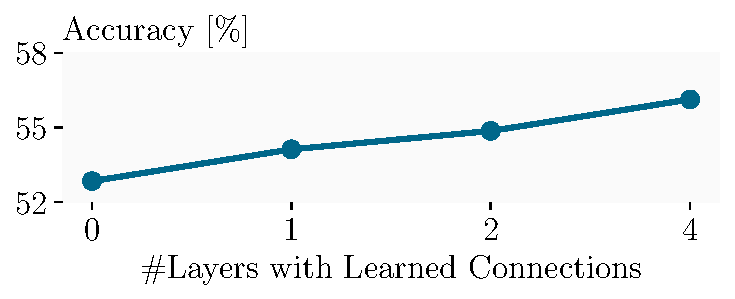
\includegraphics[width=0.7\linewidth]{figures/mip_ablation}
    \caption{The result of learning partial connections on \cifar. Note that the x-axis is unequally spaced.}
    \label{fig:mip_ablaition}
\end{figure}

\paragraph{Resampling vs More Candidates} As discussed in \cref{sec:learning_connectivity}, 
resampling aims to explore new candidates during training. 
One direct alternative is to simply increase the number of candidate triples $(\vk_i, \vp_i, \vq_i)$ per neuron, from 16 to a larger number $K$. 
Such choices naturally allows the neuron to aggregate information from a larger pool of candidates. However, we shall show that with the proposed resampling strategy, 
increasing the number of candidates is unnecessary, thereby saving computation and memory during training. 
To verify this, 
we conduct an ablation study on \cifar with the same small model, 
varying the number of candidates $K$ from 16 to 128. As shown in \cref{fig:acc_vs_k}, without resampling, increasing $K$ from 16 to 128 improves the accuracy 
clearly,
from 53.24\% to 54.94\%. 
However, with resampling, the accuracy gain becomes marginal, from 56.14\% to 56.48\%. Further, for all $K$, 
resampling consistently outperforms the non-resampling counterpart. These results validate the effectiveness of the proposed resampling strategy in exploring 
new candidates during training, thus removes the necessity of introducing more candidates and the associated memory and computational overhead.



\begin{figure}
    \centering
    \includegraphics[width=0.8\columnwidth]{figures/Acc_vs_K}
    \caption{The effect of increasing the number of candidate triples, with and without resampling. Note the log scale on x-axis.}
    \label{fig:acc_vs_k}
\end{figure}
\subsection{Convolution} \label{sec:exp_convolution}

In this part, we evaluate the proposed convolutional architecture that uses a single 
Boolean operation for the convolutional kernel, against TreeLogicNet that uses  Boolean trees for convolutional kernels. 
Both architectures %
use 3x3 receptive field.  TreeLogicNet restricts every kernel to see two neighboring channels, while we further restrict the number of channels seen by each kernel to one. 
We will show that such restriction improves performance significantly, and hypothesize that it is due to the destructive effect of thermometer encoding on natural images.

\paragraph{Main Results} The results on \mnist and \cifar are summarized in \cref{tb:CLGN_MNIST} and \cref{tb:CLGN_CIFAR}, respectively. Our architecture consistently outperforms 
TreeLogicNet with fewer neurons. On \mnist, our medium model outperforms the large TreeLogicNet with 22x fewer (520K vs 11.8M) neurons. 
On \cifar, our large model achieves 0.71\% higher accuracy (72.09\% vs 71.38\%) with 3x fewer (2.33M vs 7M) neurons than TreeLogicNet. 
We remark that larger models reported in \citet{petersen2024convolutional} are not Boolean networks since they 
contain floating-point feature extraction layers, and are thus excluded in the comparison.

\begin{table}
\centering
\caption{Comparison between TreeLogicNet and our method on MNIST.}
\label{tb:CLGN_MNIST}
  \resizebox*{.75\linewidth}{!}{%

\begin{tabular}{lccc}
\toprule
Method & Acc. & \emph{\#neurons} & \emph{\#BOPs} \\
\midrule
TreeLogicNet-S	& $97.81\%$ & 185 K & 117 K \\
TreeLogicNet-M	& $98.95\%$ & 740 K & 427 K \\
TreeLogicNet-L	& $99.32\%$ & 11.8 M & 6.20 M \\
\midrule
Ours-S	    & \textbf{$99.12\%$} & 260 K & 165 K \\
Ours-M	    & \textbf{$99.35\%$} & 520 K & 240 K \\
\bottomrule
\end{tabular}
  }
\end{table}

\begin{table}
\centering
\caption{Comparison between TreeLogicNet and our method on CIFAR-10.}
\label{tb:CLGN_CIFAR}
  \resizebox*{.75\linewidth}{!}{%

\begin{tabular}{lccc}
\toprule
Method & Acc. & \emph{\#neurons} & \emph{\#BOPs} \\
\midrule
TreeLogicNet-S	& $59.79\%$ & 874 K & 521 K \\
TreeLogicNet-M	& $71.38\%$ & 7.00 M & 3.66 M \\
\midrule
Ours-S	& \textbf{$65.85\%$} & 291 K & 174 K \\
Ours-M	& \textbf{$69.44\%$} & 582 K & 389 K \\
Ours-L	& \textbf{$72.09\%$} & 2.33 M & 1.09 M \\
\bottomrule
\end{tabular}
  }
\end{table}


\paragraph{The Paradox of Channel Restriction} We conduct an extensive study on the effect of limiting the number of channels seen by each convolutional kernel here. 
\cref{fig:ablation_chn} shows the effect of limiting the number of channels accessible to each kernel
 on \cifar with our medium model. We find a similar conclusion as in \citet{petersen2024convolutional}: limiting the number of accessible channels improves performance significantly. 
 In particular, restricting each kernel to see only one channel achieves the best accuracy, 4.56\% higher than seeing all channels (69.46\% vs 64.90\%). This phenomenon leads to a direct paradox: restricting the visible channels to one means that composition of convolutional layers 
 can no longer mix information across channels. Intuitively, this should have hurt the performance instead.
 We hypothesize that this is due to the destructive effect of thermometer encoding on natural images. As  visualized in \cref{app:thermo_effects}, thermometer encoding breaks the complementary information across channels in natural images, sometimes even completely removing the information in some channels. This might lead to interference across channels when multiple channels are seen by the same kernel. Therefore, a better input encoding scheme that preserves cross-channel information might allow efficient information composition across channels and further improve the performance of convolutional Boolean networks. We leave further exploration of this paradox to future work.


\begin{figure}
    \centering
    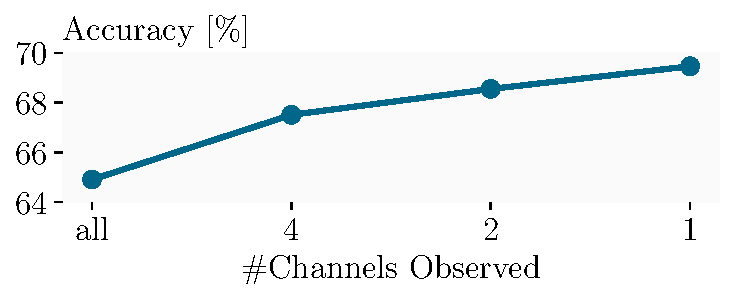
\includegraphics[width=0.73\linewidth]{figures/num_ablation}
    \caption{The effect of limiting the number of channels seen by each convolutional kernel on \cifar. Note that the x-axis is unequally spaced.}
    \label{fig:ablation_chn}
\end{figure}



\subsection{Adaptive Discretization} \label{sec:exp_discretization}

In this part, we evaluate the proposed adaptive discretization strategy, comparing it against Gumbel noise injection. In addition to test accuracy, we also measure the discretization gap, defined as the accuracy difference between the relaxed model before discretization and the discretized Boolean network after discretization, following \citet{yousefi2025mind}.

\begin{figure}
    \centering
    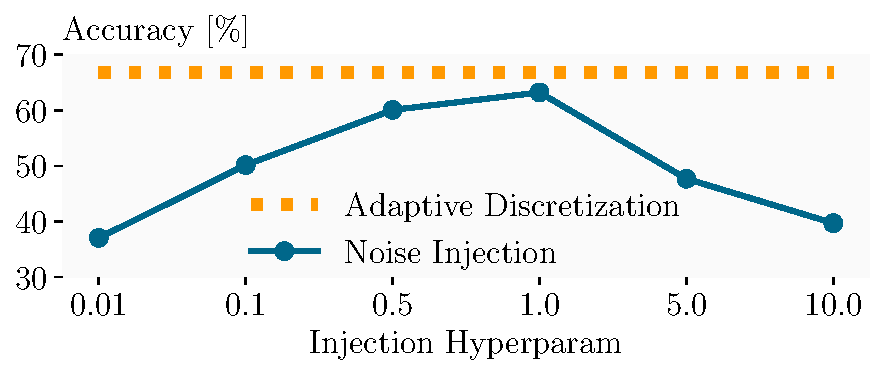
\includegraphics[width=0.85\columnwidth]{figures/gumbel_vs_lh}
    \caption{Comparison between noise injection and the proposed adaptive discretization. Note that the x-axis is unequally spaced.}
    \label{fig:gumbel_vs_lh}
\end{figure}

\paragraph{Main Results} \cref{fig:gumbel_vs_lh} compares the proposed adaptive discretization against Gumbel noise injection on \cifar with our medium convolutional model. We sweep the hyperparameter for Gumbel noise injection for a fair comparison. As shown in \cref{fig:gumbel_vs_lh}, our method consistently outperforms Gumbel noise injection in test accuracy. Further, the adaptive discretization significantly reduces the training cost, since discretized layers are more efficient in both forward and backward passes. For example, after discretizing four convolutional layers, the model trains 1.8x faster than the original model. In contrast, Gumbel noise injection leads to computational overhead throughout training.

\paragraph{Adaption Reduces Discretization Gap Progressively} We conduct an ablation study on \cifar with our medium convolutional model, varying the number of layers discretized during training from 1 to 5 (the model has 6 layers in total). As shown in \cref{fig:acc_vs_frozen_layers}, progressively discretizing more layers during training consistently reduces the discretization gap, 
demonstrating the effectiveness of the proposed adaptive discretization strategy. However, due to the limited number of training steps, progressively discretizing all layers during training does not lead to the best accuracy after discretization, as the model has insufficient resource to learn better solutions. In practice, we find that progressively discretizing all convolutional layers works well for all models, achieving a good balance between reducing the discretization gap and allowing sufficient learning. This is possibly because non-convolutional layers can converge steadily without discretization during training (c.f. \cref{fig:row_argmax_difference}). Therefore, for our final models, we always adaptively discretize all convolutional layers, as described in \cref{sec:adaptive_discretization}.

\begin{figure}
    \centering
    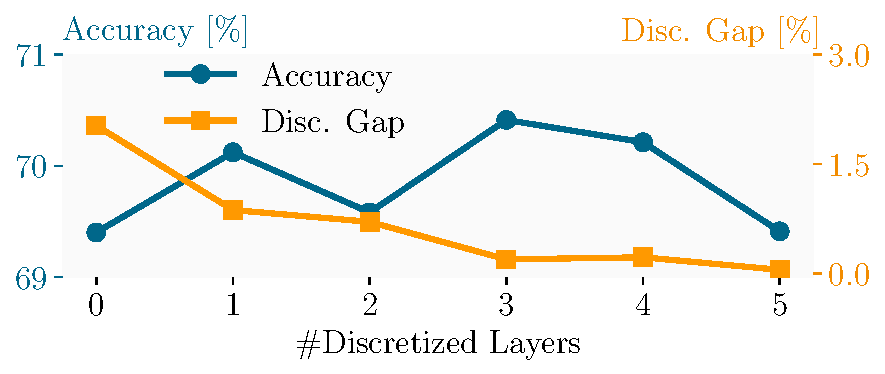
\includegraphics[width=0.85\linewidth]{figures/disc_gap_vs_frozen_layers}
    \caption{The effect of the number of discretized layers during training on the accuracy and discretization gap.}
    \label{fig:acc_vs_frozen_layers}
    \vspace{-1em}
\end{figure}

\subsection{Combined Results} \label{sec:exp_main}
We combine all proposed methods together and evaluate the final performance on \mnist and \cifar. The results are summarized in \cref{tb:exp_main}. On \mnist, our small and medium models achieve 99.35\% and 99.41\% accuracy, outperforming the large TreeLogicNet with 45x and 22x fewer neurons (260K and 520K vs 11.8M), respectively. After pruning, our models demonstrate a reduction in \#BOPs by 37x and 27x (168K and 228K vs 6.2M), respectively. On \cifar, our large model achieves 72.67\% accuracy, outperforming TreeLogicNet with 3x fewer neurons and \#BOPs. We further report the performance variance over random seeds in \cref{app:variance_seeds}. These results validate the effectiveness and stability of the proposed methods in learning compact and accurate Boolean networks.

\begin{table}
\centering
\caption{The comparison between our final models and the state-of-the-art TreeLogicNet.}
\label{tb:exp_main}
\resizebox{\columnwidth}{!}{
\begin{tabular}{llccc}
\toprule
Dataset	& Method & Acc. & \emph{\#neurons} & \emph{\#BOPs} \\
\midrule
\multirow{5}{*}{MNIST}
& TreeLogicNet-S	& $97.81\%$ & 185 K & 117 K \\
& TreeLogicNet-M	& $98.95\%$ & 740 K & 427 K \\
& TreeLogicNet-L	& $99.32\%$ & 11.8 M & 6.20 M \\
\cmidrule(l){2-5}
& Ours-S	    & \textbf{$99.35\%$} & 260 K & 168 K \\
& Ours-M	    & \textbf{$99.41\%$} & 520 K & 228 K \\
\midrule
\multirow{5}{*}{CIFAR-10}
& TreeLogicNet-S	& $59.79\%$ & 874 K & 521 K \\
& TreeLogicNet-M	& $71.38\%$ & 7.00 M & 3.66 M \\
\cmidrule(l){2-5}
& Ours-T	& \textbf{$62.34\%$} & 145 K & 100 K \\
& Ours-S	& \textbf{$66.92\%$} & 291 K & 197 K \\
& Ours-M	& \textbf{$70.21\%$} & 582 K & 337 K \\
& Ours-L	& \textbf{$72.67\%$} & 2.33 M & 1.08 M \\
\bottomrule
\end{tabular}
}
\end{table}

\vspace{-1em}
